\documentclass[addpoints, 12pt]{exam}

\usepackage{amsmath}
\usepackage{tikz}
%\usepackage[latin1]{inputenc}
\usetikzlibrary{shapes,arrows}
\usetikzlibrary{calc,arrows,through}
\usetikzlibrary{intersections}
\usepackage{multicol}


\pagestyle{empty}

\tikzstyle{line} = [draw, -triangle 45]

\newcommand{\perpbox}[3]{
	\draw ($(#1)!.3cm!(#2)$)--($($(#1)!.3cm!(#2)$)!.3cm!90:(#2)$)--($(#1)!.3cm!(#3)$);
}

\newcommand{\linedraw}[2]{
	\draw [line] (#2)--($(#2)!.5cm!180:(#1)$);
	\draw [line] (#2)--($(#1)!.5cm!180:(#2)$);
}

\newcommand{\raydraw}[2]{
	\draw [line] (#1)--($(#2)!.5cm!180:(#1)$);
}

\newcommand{\fillpoints}[1]{
	\foreach \point in {#1} \fill (\point) circle (2.5pt);
}

\begin{document}

\begin{tabbing}
\noindent Name: \rule[-0.1cm]{5cm}{0.01cm} \hspace{2.5in} \=  \\
Precalculus*: Unit Circle Worksheet  
\end{tabbing}

\begin{questions}

\question Fill in the missing side lengths on the triangles below.

\begin{center}
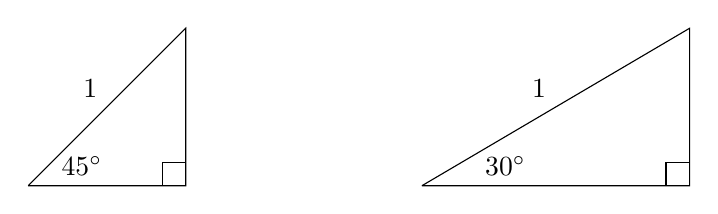
\begin{tikzpicture}

\draw (0,0)--(2,0) node [above right, pos=0.15] {$45^\circ$}--(2,2)--(0,0) node [above left, pos=0.5] {1};
\draw (5,0)--(8.4,0) node [above right, pos=0.2] {$30^\circ$}--(8.4,2)--(5,0) node [above left, pos=0.5] {1};
\perpbox {2,0}{2,2}{0,0}
\perpbox {8.4,0}{8.4,2}{5,0}

\end{tikzpicture}
\end{center}

\question Fill in the missing coordinates on the unit circle below.


\begin{center}
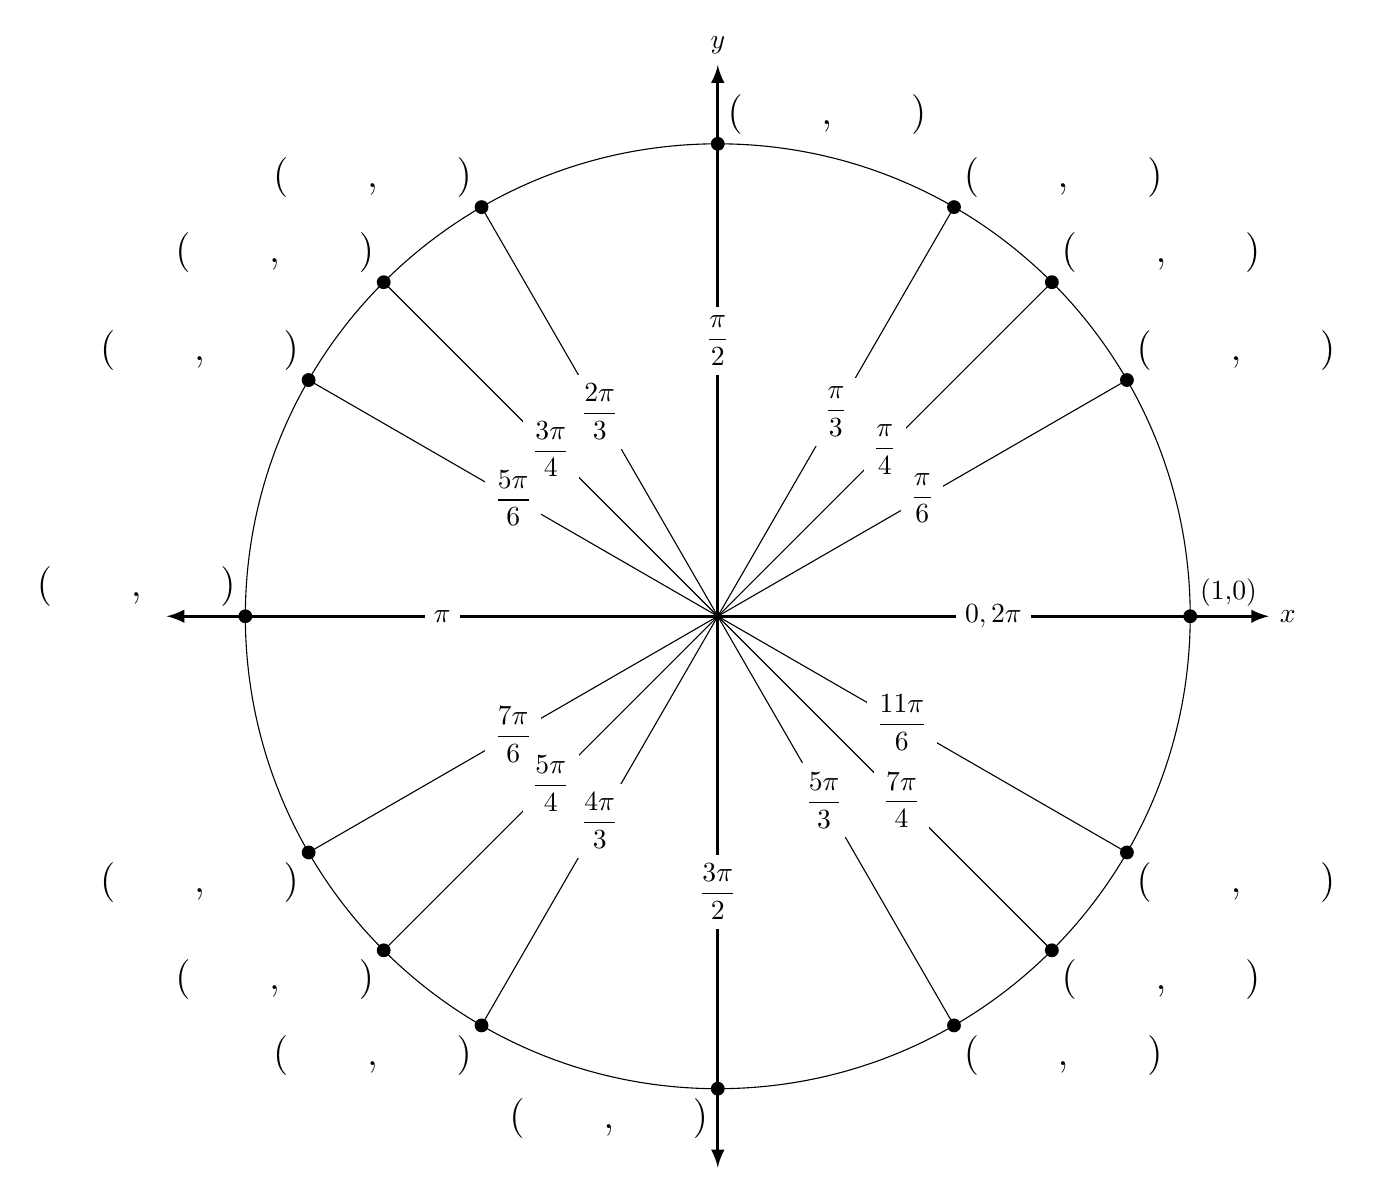
\begin{tikzpicture}
\draw [latex-latex,very thick] (-7,0)--(7,0) node [right] {$x$} node [pos=0.25,fill=white]{$\pi$} node [pos=0.75,fill=white]{$0,2\pi$};
\draw [latex-latex,very thick] (0,-7)--(0,7) node [above] {$y$} node [pos=0.25,fill=white]{$\dfrac{3\pi}{2}$} node [pos=0.75,fill=white]{$\dfrac{\pi}{2}$};
\coordinate (X)	at (0,0);
\draw (X) circle (6cm);
\coordinate [label=above right:{(1,0)}]	(A)	at (0:6);
\coordinate [label=above right:{{\Large (\hspace{1cm},\hspace{1cm})}}]	(B)	at (30:6);
\coordinate [label=above right:{{\Large (\hspace{1cm},\hspace{1cm})}}]	(C)	at (45:6);
\coordinate [label=above right:{{\Large (\hspace{1cm},\hspace{1cm})}}]	(D)	at (60:6);
\coordinate [label=above right:{{\Large (\hspace{1cm},\hspace{1cm})}}]	(N)	at (90:6);

\coordinate [label=above left:{{\Large (\hspace{1cm},\hspace{1cm})}}]	(E)	at (120:6);
\coordinate [label=above left:{{\Large (\hspace{1cm},\hspace{1cm})}}]	(F)	at (135:6);
\coordinate [label=above left:{{\Large (\hspace{1cm},\hspace{1cm})}}]	(G)	at (150:6);
\coordinate [label=above left:{{\Large (\hspace{1cm},\hspace{1cm})}}]	(O)	at (180:6);

\coordinate [label=below left:{{\Large (\hspace{1cm},\hspace{1cm})}}]	(H)	at (210:6);
\coordinate [label=below left:{{\Large (\hspace{1cm},\hspace{1cm})}}]	(I)	at (225:6);
\coordinate [label=below left:{{\Large (\hspace{1cm},\hspace{1cm})}}]	(J)	at (240:6);
\coordinate [label=below left:{{\Large (\hspace{1cm},\hspace{1cm})}}]	(P)	at (270:6);

\coordinate [label=below right:{{\Large (\hspace{1cm},\hspace{1cm})}}]	(K)	at (300:6);
\coordinate [label=below right:{{\Large (\hspace{1cm},\hspace{1cm})}}]	(L)	at (315:6);
\coordinate [label=below right:{{\Large (\hspace{1cm},\hspace{1cm})}}]	(M)	at (330:6);

\draw (X)--(B) node [pos=0.5,fill=white]{$\dfrac{\pi}{6}$};
\draw (X)--(C) node [pos=0.5,fill=white]{$\dfrac{\pi}{4}$};
\draw (X)--(D) node [pos=0.5,fill=white]{$\dfrac{\pi}{3}$};

\draw (X)--(E) node [pos=0.5,fill=white]{$\dfrac{2\pi}{3}$};
\draw (X)--(F) node [pos=0.5,fill=white]{$\dfrac{3\pi}{4}$};
\draw (X)--(G) node [pos=0.5,fill=white]{$\dfrac{5\pi}{6}$};

\draw (X)--(H) node [pos=0.5,fill=white]{$\dfrac{7\pi}{6}$};
\draw (X)--(I) node [pos=0.5,fill=white]{$\dfrac{5\pi}{4}$};
\draw (X)--(J) node [pos=0.5,fill=white]{$\dfrac{4\pi}{3}$};

\draw (X)--(K) node [pos=0.45,fill=white]{$\dfrac{5\pi}{3}$};
\draw (X)--(L) node [pos=0.55,fill=white]{$\dfrac{7\pi}{4}$};
\draw (X)--(M) node [pos=0.45,fill=white]{$\dfrac{11\pi}{6}$};

\fillpoints {A,B,C,D,E,F,G,H,I,J,K,L,M,N,O,P};
\end{tikzpicture}
\end{center}

\newpage

\question Fill in the table below.

\renewcommand{\arraystretch}{2.3}
		\begin{center}
		\begin{tabular}{|@{\hspace{0.5cm}}c @{\hspace{0.5cm}}| @{\hspace{0.2cm}} c @{\hspace{0.2cm}}|  
			@{\hspace{0.5cm}}c @{\hspace{0.5cm}} | @{\hspace{0.5cm}}c @{\hspace{0.5cm}} |  @{\hspace{0.5cm}} c @{\hspace{0.5cm}}|} \hline 
		$\theta$&$\theta$ (in degrees) &sin $\theta$&cos $\theta$&tan $\theta$\\ \hline
		0 &&&&\\	\hline
		$\dfrac{\pi}{6}$ &&&&\\	\hline
		$\dfrac{\pi}{4}$ &&&&\\	\hline
		$\dfrac{\pi}{3}$ &&&&\\	\hline
		$\dfrac{\pi}{2}$ &&&&\\	\hline
		$\dfrac{2\pi}{3}$ &&&&\\	\hline
		$\dfrac{3\pi}{4}$ &&&&\\	\hline
		$\dfrac{5\pi}{6}$ &&&&\\	\hline
		$\pi$ &&&&\\	\hline
		$\dfrac{7\pi}{6}$ &&&&\\	\hline
		$\dfrac{5\pi}{4}$ &&&&\\	\hline
		$\dfrac{4\pi}{3}$ &&&&\\	\hline
		$\dfrac{3\pi}{2}$ &&&&\\	\hline
		$\dfrac{5\pi}{3}$ &&&&\\	\hline
		$\dfrac{7\pi}{4}$ &&&&\\	\hline
		$\dfrac{11\pi}{6}$ &&&&\\	\hline
		$2\pi$ &&&&\\	\hline
		
		\end{tabular}
		\end{center}
		
	

\end{questions}

\end{document}